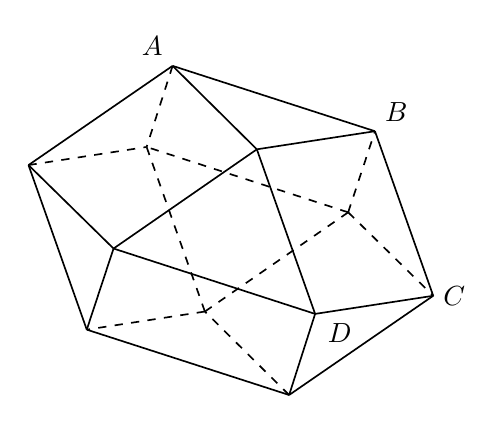
\begin{tikzpicture}[line width=.6pt]
% cuboctahedron: 3D vertices (x,y,z) in {+-1} combos, orthographic
% X=(z-x)*1.35, Y=((x+z)*0.4-0.9y)*1.35; back edges (avg depth<-0.3) dashed
\coordinate (v0) at (-1.49,-0.23); % (1,1,0)
\coordinate (v1) at (-0.74,2.09); % (1,-1,0) = A
\coordinate (v2) at (0.74,-2.09); % (-1,1,0)
\coordinate (v3) at (1.49,0.23); % (-1,-1,0)
\coordinate (v4) at (0.33,1.03); % (1,0,1)
\coordinate (v5) at (-2.57,0.83); % (1,0,-1)
\coordinate (v6) at (2.57,-0.83); % (-1,0,1) = C
\coordinate (v7) at (-0.33,-1.03); % (-1,0,-1)
\coordinate (v8) at (1.07,-1.06); % (0,1,1) = D
\coordinate (v9) at (-1.83,-1.26); % (0,1,-1)
\coordinate (v10) at (1.83,1.26); % (0,-1,1) = B
\coordinate (v11) at (-1.07,1.06); % (0,-1,-1)
% solid visible edges
\draw (v0) -- (v4);
\draw (v0) -- (v5);
\draw (v0) -- (v8);
\draw (v0) -- (v9);
\draw (v1) -- (v4);
\draw (v1) -- (v5);
\draw (v1) -- (v10);
\draw (v2) -- (v6);
\draw (v2) -- (v8);
\draw (v2) -- (v9);
\draw (v4) -- (v8);
\draw (v4) -- (v10);
\draw (v5) -- (v9);
\draw (v6) -- (v8);
\draw (v6) -- (v10);
% hidden edges
\draw[dashed] (v1) -- (v11);
\draw[dashed] (v2) -- (v7);
\draw[dashed] (v3) -- (v6);
\draw[dashed] (v3) -- (v7);
\draw[dashed] (v3) -- (v10);
\draw[dashed] (v3) -- (v11);
\draw[dashed] (v5) -- (v11);
\draw[dashed] (v7) -- (v9);
\draw[dashed] (v7) -- (v11);
% labels
\node[above left] at (v1) {$A$};
\node[above right] at (v10) {$B$};
\node[right] at (v6) {$C$};
\node[below right,xshift=1pt] at (v8) {$D$};
\end{tikzpicture}
